
%(BEGIN_QUESTION)
% Copyright 2014, Tony R. Kuphaldt, released under the Creative Commons Attribution License (v 1.0)
% This means you may do almost anything with this work of mine, so long as you give me proper credit

I denne grafen med to AC-spenninger, hvilken {\it leder} og hvilken {\it henger etter}?

$$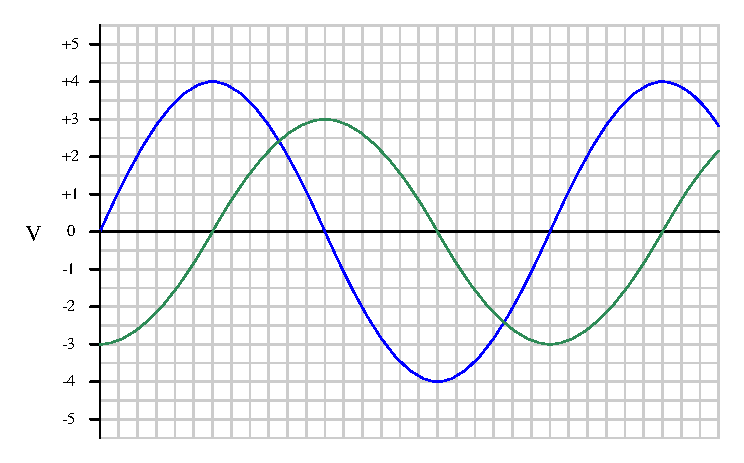
\includegraphics[width=15.5cm]{i00839x01.eps}$$

Hvis sinuskurven med 4 V (toppverdi) skrives i fasornotasjon som $4 \hbox{ V} \angle \> 0^o$, hvordan skal sinuskurven med 3 V (toppverdi) skrives? Oppgi både polar og rektangulær form.

\vskip 5pt

Hvis sinuskurven med 4 V (toppverdi) skrives i fasornotasjon som $4 \hbox{ V} \angle \> 90^o$, hvordan skal sinuskurven med 3 V (toppverdi) skrives? Oppgi både polar og rektangulær form.

\underbar{file i00839}
%(END_QUESTION)





%(BEGIN_ANSWER)

Bølgeformen på 4 volt (topp) {\it leder} bølgeformen på 3 volt (topp). Omvendt {\it henger} 3-voltsbølgen etter 4-voltsbølgen.

\vskip 5pt

Hvis 4-voltsbølgen skrives som 4 V $\angle$ 0$^o$, skal 3-voltsbølgen skrives som 3 V $\angle$ $-90^o$, eller $0 - j3$ V.

\vskip 5pt

Hvis 4-voltsbølgen skrives som 4 V $\angle$ 90$^o$ ($0 + j4$ V i rektangulær form), skal 3-voltsbølgen skrives som 3 V $\angle$ 0$^o$, eller $3 + j0$ V.


%(END_ANSWER)





%(BEGIN_NOTES)


%INDEX% Electricity review: phase shift measurement (dual-trace oscilloscope)

%(END_NOTES)
